\chapter{Model Architecture}

In this chapter, the architectures of several models are presented. Section \ref{modpoly} gives a comprehensive explanation to the structure of PolygonRNN, while section \ref{modrcnn} looks into the FPN part of Mask R-CNN. Considering our problem, we combine PolygonRNN and FPN part of Mask R-CNN together and come up with a new model, which is called \modelnameshort\ (\modelnamelong, see section \ref{modmer}). In theory, the proposed model can find out the bounding boxes of buildings within an aerial image and give geometrical shape for each building.
 
\section{PolygonRNN}\label{modpoly}

PolygonRNN is the core model for finding geometrical shapes in this project. Figure \ref{fig:simppoly} shows the simplified structure of PolygonRNN. The CNN part (see subsection \ref{modcnn}) can capture image features through multilayer convolutions and max pooling, which is then fed into the RNN part (see subsection \ref{modrnn}) to sequentially find out the polygon vertices.

\begin{figure}[!h]
	\centering
	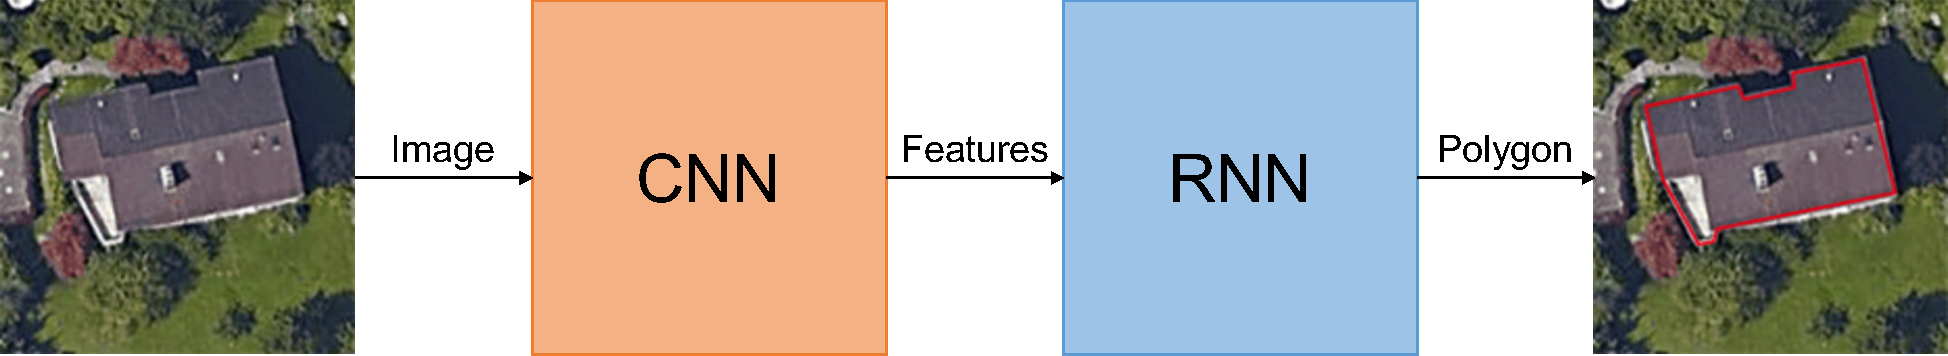
\includegraphics[width=\fig\textwidth]{3-00.pdf}
    \caption[The simplified model architecture of PolygonRNN]{The simplified model architecture of PolygonRNN.}
    \label{fig:simppoly}
\end{figure}

\subsection{CNN Part}\label{modcnn}

As mentioned in subsection \ref{relatpoly}, the CNN part of PolygonRNN uses VGG-16. Actually, VGG-16 is a form of VGGNet, which is proposed by the Visual Geometry Group of Oxford University. VGGNet is very structured and focusing on deepening the  neural network without a large number of parameters. It generally believes that deeper networks have stronger expressive capabilities than shallow networks, and can accomplish more complex tasks. It also proven in practice that VGGNet has made great progress in performance compared to its previous network architecture (e.g. AlexNet).

The `16' in VGG-16 means that it is a VGGNet with 16 layers containing parameters (13 convolutional layers and 3 fully connected layers). It has around 138 million parameters in total. Figure \ref{fig:vgg16} shows its detailed network structure. From the figure we can see that VGG-16 continuously does convolution with $3\times3$ small kernels and makes $2\times2$ max pooling. As the network deepens, the width and height of the image are reduced by half after each max pooling, and the number of channels is also doubly increasing after some convolution.

\begin{figure}[!h]
	\centering
	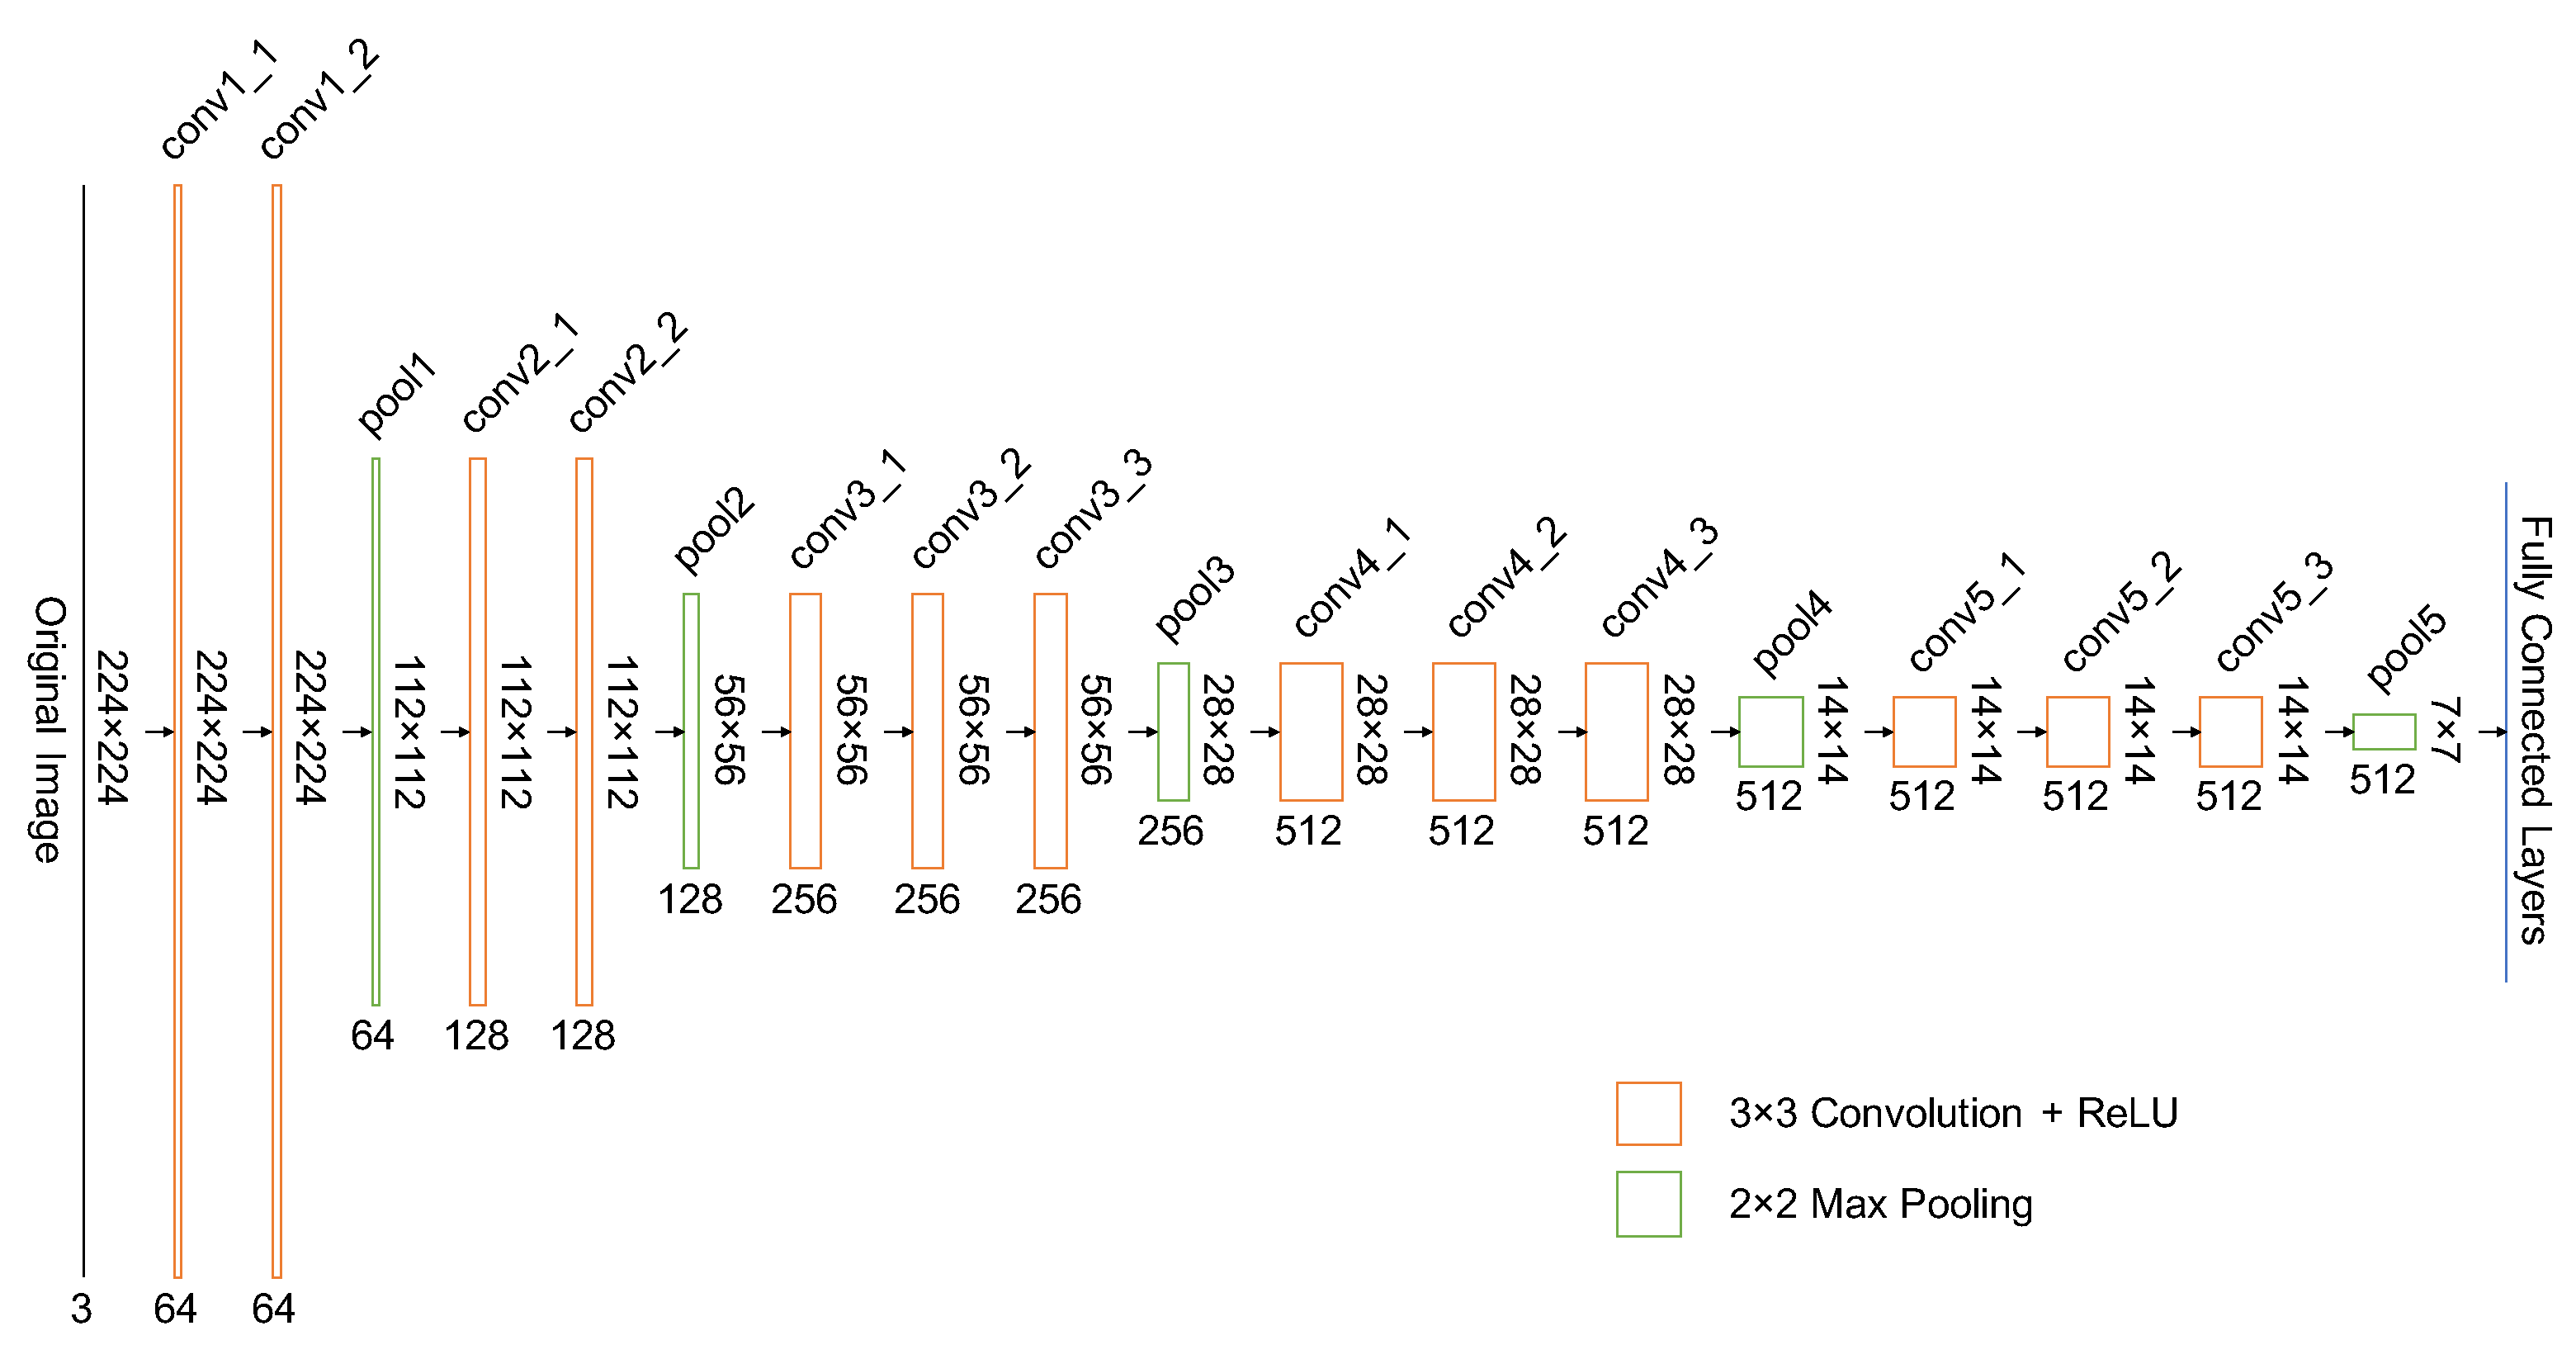
\includegraphics[width=\fig\textwidth]{3-01.pdf}
    \caption[VGG-16 architecture]{VGG-16 architecture. Only convolutional layers and maximum pooling layers are presented.}
    \label{fig:vgg16}
\end{figure}

VGG-16 was mostly used for image classification before, so after the convolutional layers and max pooling layers there are fully connected layers and softmax layer for the class labels. However, these two kinds of layers are not required for VGG-16 used in PolygonRNN, because the CNN here is working as a feature extractor and mask predictor. Layer \lstinline{pool5} is omitted as well because of the too low resolution.

\paragraph{Feature Extraction} The modified VGG-16 provides RNN with useful features, which are taken from different convolutional and max pooling layers. Specifically, the features are extracted from layer \lstinline{pool2}, \lstinline{pool3}, \lstinline{conv4_3} and \lstinline{conv5_3}. Note that since the resolution of final features is fixed, when taking features from layer \lstinline{pool2} and \lstinline{conv5_3}, it requires another max pooling and upsampling respectively. All of these can be seen in figure \ref{fig:mdfvgg16}.

\begin{figure}[!h]
	\centering
	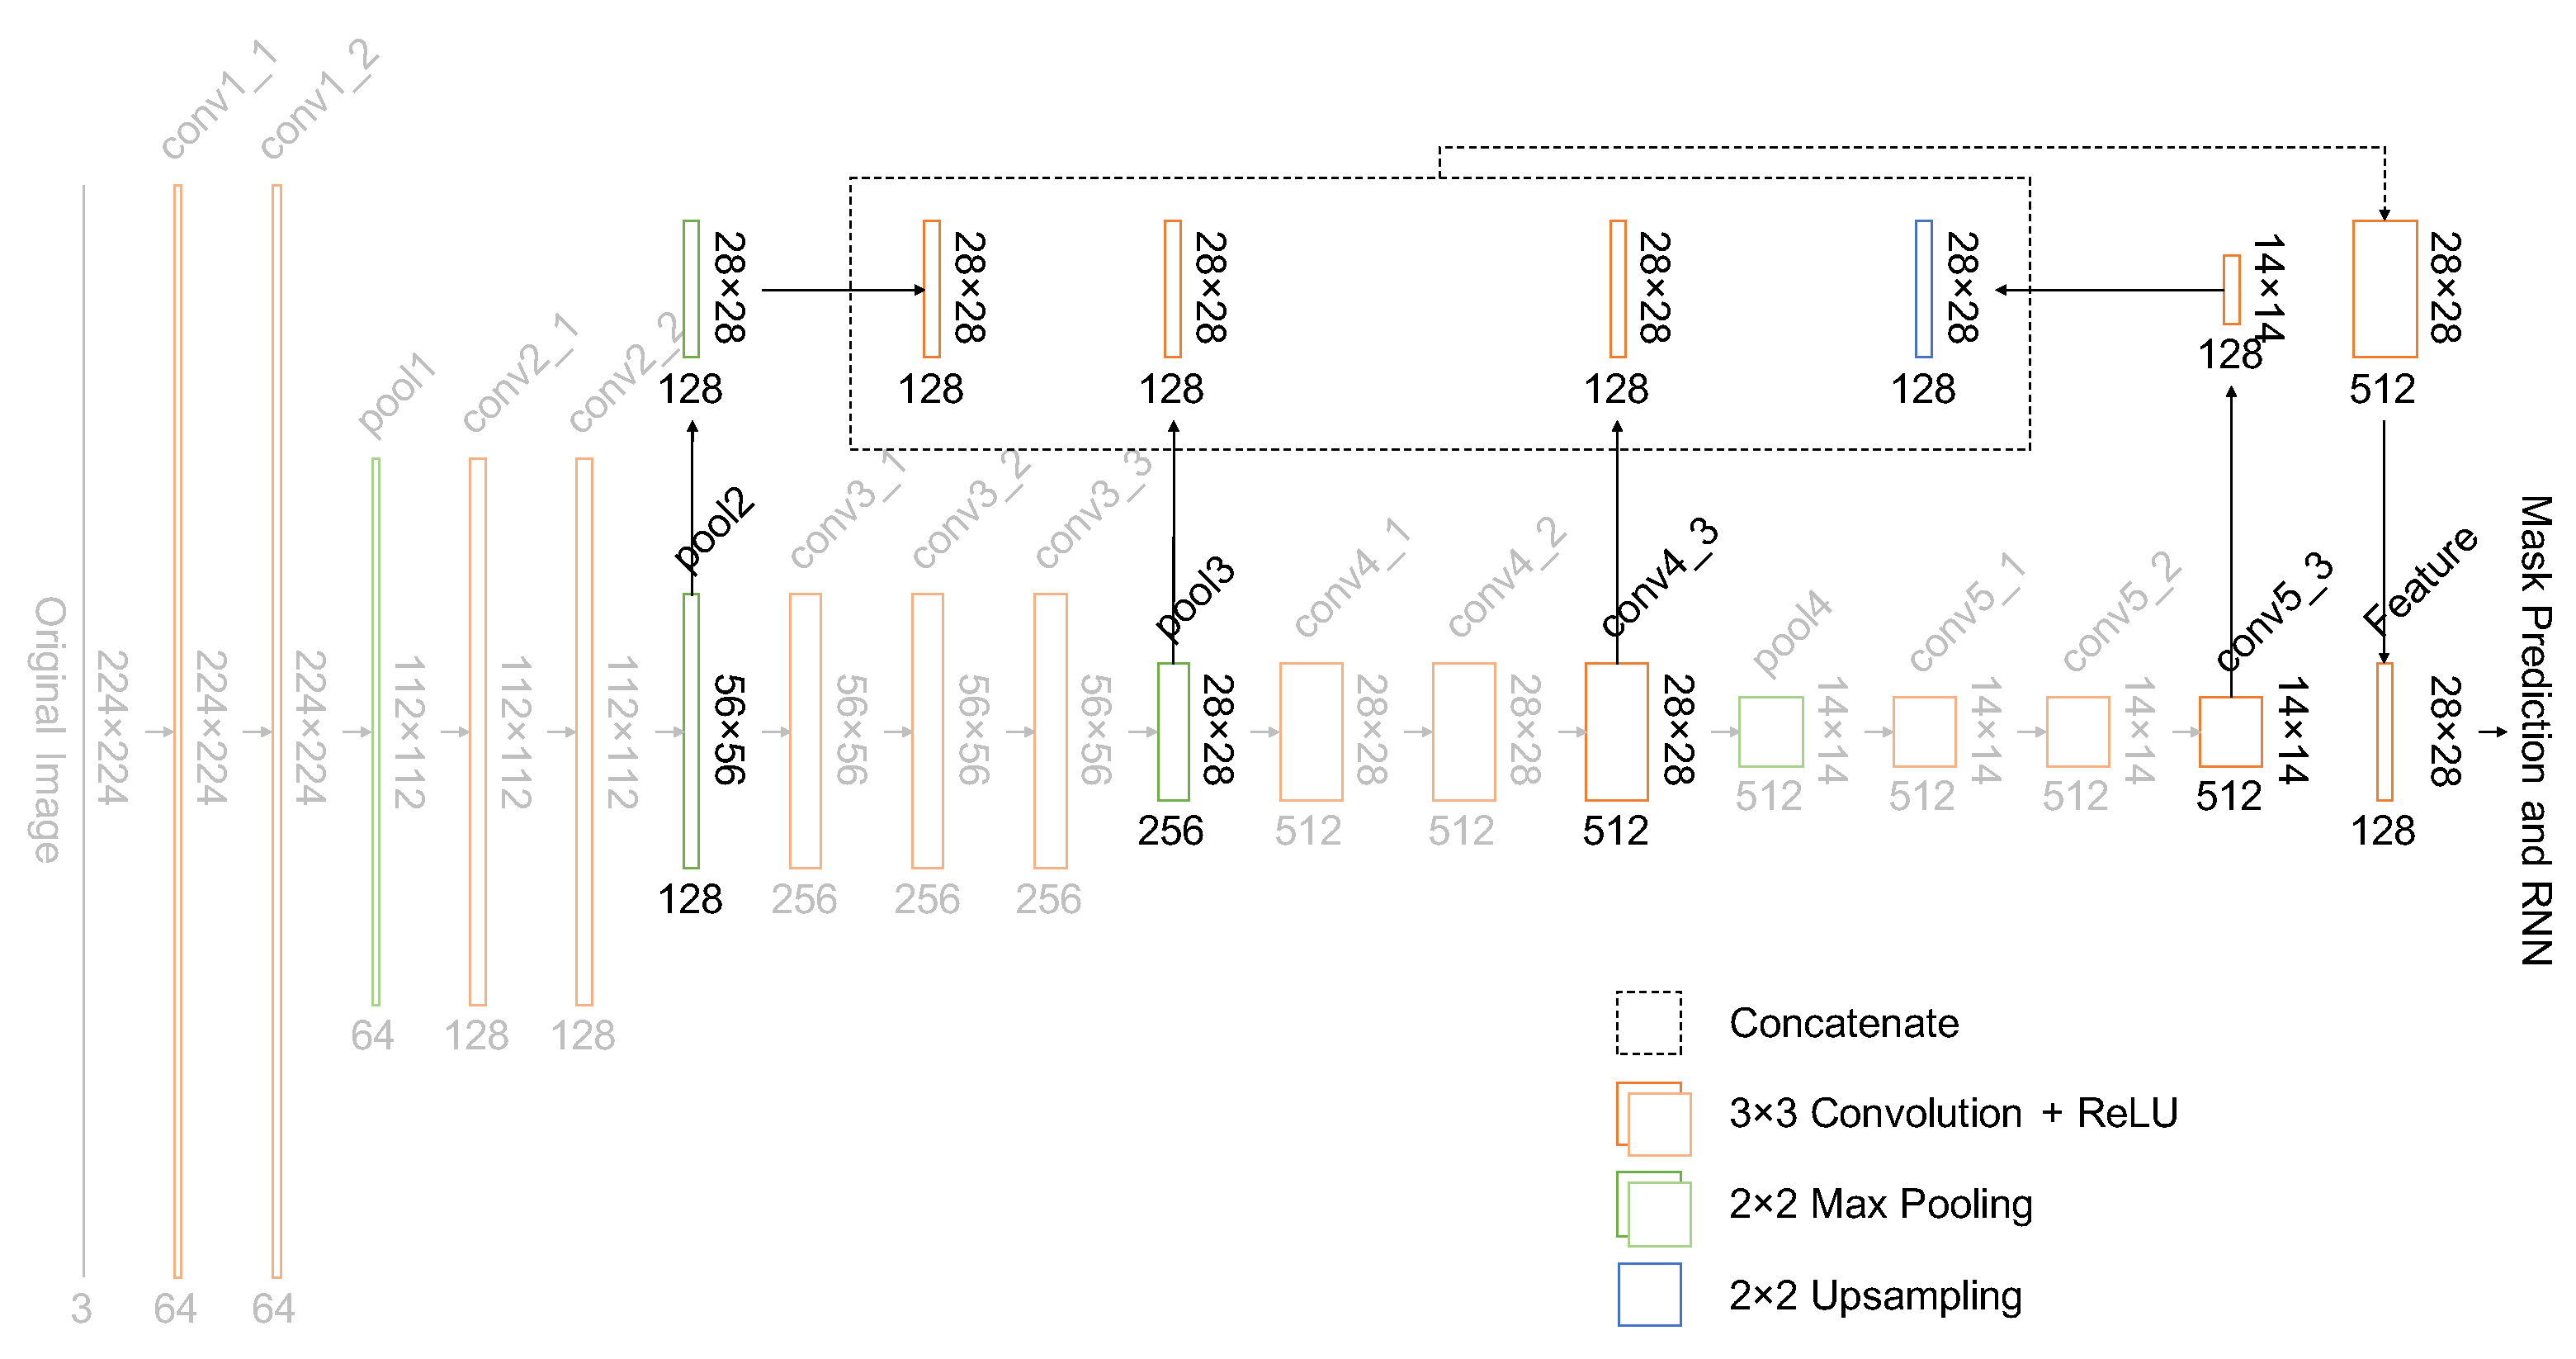
\includegraphics[width=\fig\textwidth]{3-02.pdf}
    \caption{Modified VGG-16 architecture in PolygonRNN.}
    \label{fig:mdfvgg16}
\end{figure}

\paragraph{Mask Prediction}
Another function of the CNN part is to predict masks of boundary and vertices in a low resolution (one eighth of the original). Figure \ref{fig:vgg16mask} shows the mask prediction phase. Different from the ReLU function used in the former convolutional layers, the activation function used here is the sigmoid function. Each entry of the boundary or the vertices mask indicates the probability that the pixel is located in the boundary or is a vertex respectively. The features and two masks are then sent into RNN together. As for the loss function, weighted log loss is used, given the ground truth masks of boundary and vertices.
\begin{figure}[!h]
	\centering
	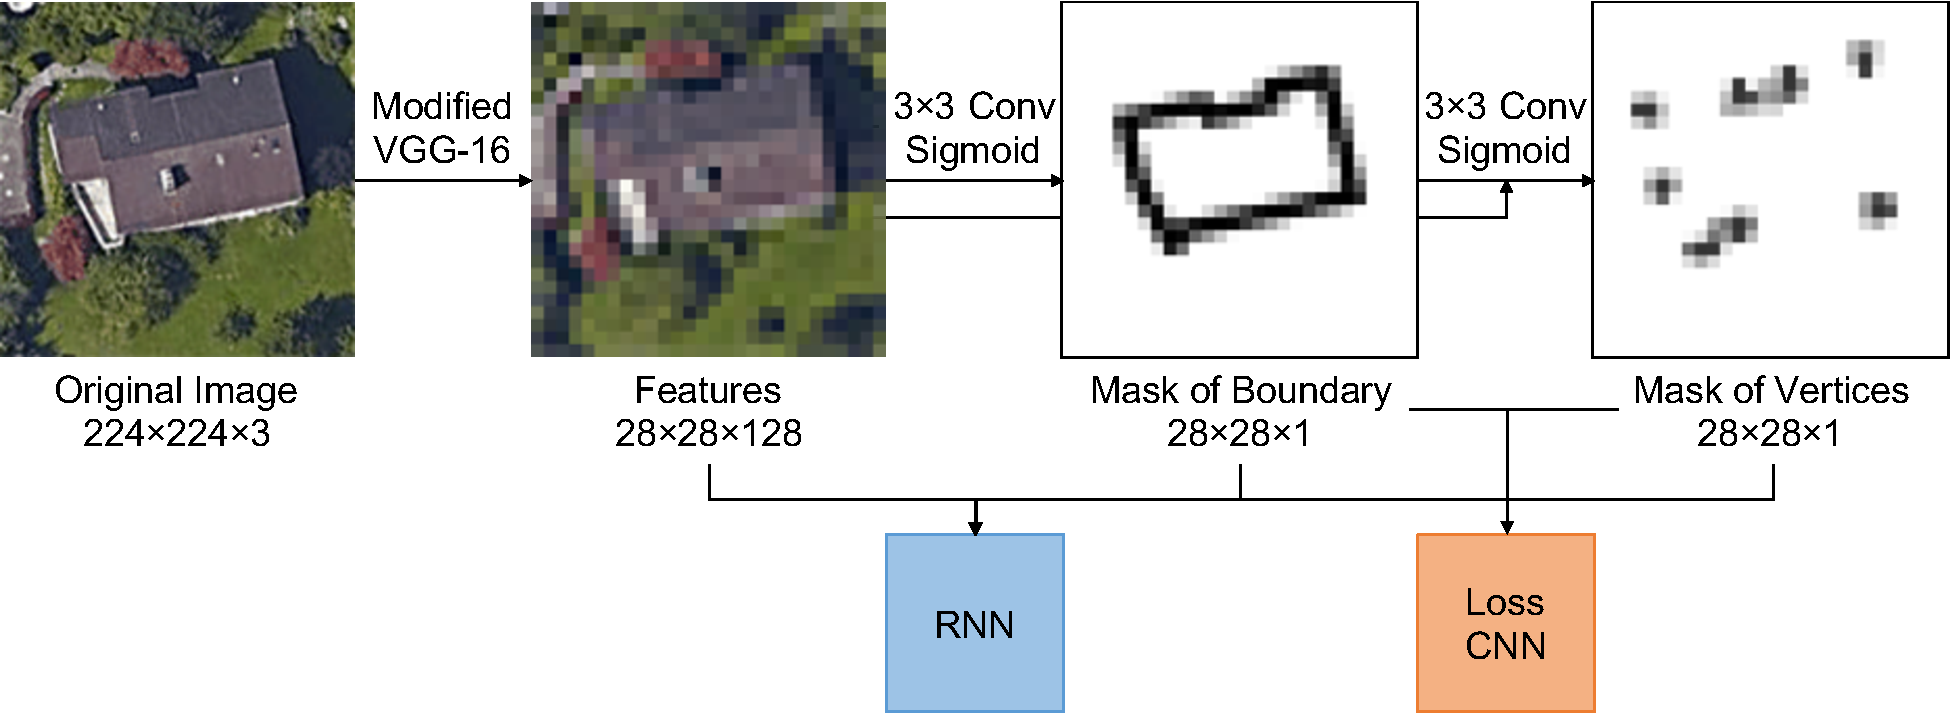
\includegraphics[width=\fig\textwidth]{3-03.pdf}
    \caption[Mask prediction of VGG-16]{Mask prediction of VGG-16. Note that the mask of vertices is obtained by the convolution on the concatenation of the features and the mask of boundary.}
    \label{fig:vgg16mask}
\end{figure}

\subsection{RNN Part}\label{modrnn}
The model used for predicting polygon vertices is RNN. We have mentioned in subsection \ref{relatpoly} that RNN is very powerful when data is related to time series, and in our case, we regards the polygon as a series of vertices. We know that given two vertices on a polygon in an order (either clockwise or anticlockwise), the third vertex after the two points can be uniquely determined. What RNN here can do is to predict the probability distribution of the next vertex's position in a low resolution when given the image features, the history information about the two vertices before, as well as the position of the starting vertex, which can be formulated as follows.
\begin{equation}\label{vnext}
	p(x_t|x_{t-1}, x_{t-2}) = F(x_{t-1}, x_{t-2}, x_{0}, p), t \in \{2,3,4,...\},
\end{equation}
where $x_t$ represents the vertex position at $t$-th prediction, $p$ is the extracted features by CNN, $F$ is a function for computing the conditional probability.

The end signal for the closure of polygon is also embedded in $x_t$, just like the `end of sentence' symbol \lstinline{<eos>} or \lstinline{</s>} in the RNN language model. Thus, $x_t$'s assignment can have $28\times28+1=785$ possible values. If the current prediction is the same as, or very close to the starting vertex $x_0$, $x_t$ will be forced to raise the end signal and the prediction of the entire polygon is then complete. Note that the conditional probability (equation \ref{vnext}) requires the first vertex when calculation, as it tells the model when to finish the prediction phase.

However, two special cases $p(x_0)$ and $p(x_1|x_0)$ are not included in equation \ref{vnext}. These two cases are different from the general case, and should be considered in addition. In particular, we can directly regard the mask of vertices (for example, the rightmost image in figure \ref{fig:vgg16mask}) predicted by the CNN as $x_0$'s unnormalized probability distribution $\tilde{p}(x_0)$, and choose the position with the highest probability for $x_0$'s assignment. As $x_0$ is known, there are typically two options for $x_1$, one on the left side and one on the right side. To tackle this problem, we can simply specify the order of the polygon vertices to be clockwise so that $x_1$ can be uniquely determined.

Figure XXX gives a Cell
  模型是一个RNN,每一次迭代预测一个多边形顶点。RNN每一次迭代的输入it包含以下三个方面。
第一是图片的CNN特征表示;
第二是前两个RNN迭代输出的顶点yt−1和yt−2,依一个特殊方向形成多边形;
第三是起点,帮助RNN决定何时封闭多边形。整个网络框架如下图:





\paragraph{ConvLSTM}
In particular, we employ a Convolutional LSTM [30] in
our model, and use it as a decoder. ConvLSTMs operate in 2D, which allows us to preserve the spatial information received from the CNN. Furthermore, a ConvLSTM em- ploys convolutions, thus greatly reducing the number of pa- rameters to be learned compared to using a fully-connected RNN. In its simplest form, a ConvLSTM (single layer) computes the hidden state ht given the input xt according to the following equations:
\begin{equation}
	\left[\begin{array}{c}
		f_t\\i_t\\g_t\\o_t
	\end{array}\right] = \left[\begin{array}{c}
		W_{hf}\\W_{hi}\\W_{hg}\\W_{ho}
	\end{array}\right] * h_{t-1} + \left[\begin{array}{c}
		W_{xf}\\W_{xi}\\W_{xg}\\W_{xo}
	\end{array}\right] * x_{t} + \left[\begin{array}{c}
		b_f\\b_i\\b_g\\b_o
	\end{array}\right] = W_h * h_{t-1} + W_x * x + b
\end{equation}
\begin{equation}
	c_t = \sigma(f_t) \circ c_{t-1} + \sigma(i_t) \circ \tanh(g_t)
\end{equation}
\begin{equation}
	h_t = \sigma(o_t) \circ \tanh(c_t)
\end{equation}

\ref{fig:lstmcell}
\begin{figure}[!h]
	\centering
	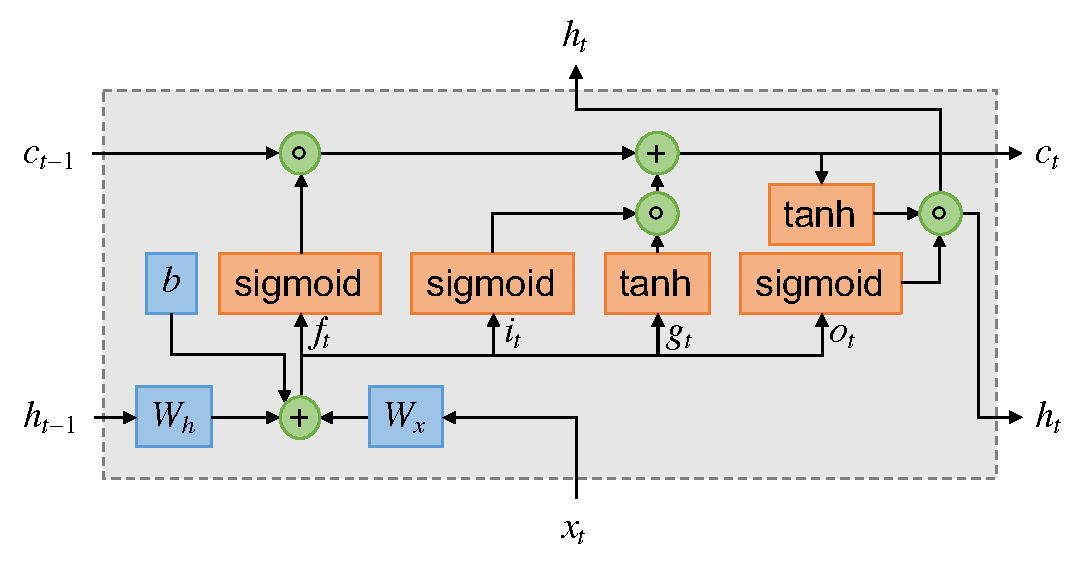
\includegraphics[width=\fig\textwidth]{3-04.pdf}
    \caption{Visulization for LSTM cell.}
    \label{fig:lstmcell}
\end{figure}

  文中RNN使用的是一个ConvolutionalLSTM框架,详细来说,作者设计了一个核为3*3和16通道的两层ConvLSTM框架,然后在每一步迭代就输出一个顶点yt。当给定输入图像表示xt,一个ConvLSTM单层的隐层ht计算如下:


这里写图片描述
It uses the convolutional LSTM, to sequentially produce vertices, which can be seen in the green box.

ConvLSTM

\section{Faster/Mask R-CNN}\label{modrcnn}

Dummy text.

\subsection{Region Proposal Network}\label{modrpn}

Dummy text.

\subsection{Feature Pyramid Network}\label{modfpn}

Dummy text.

\section{\modelnameshort}\label{modmer}

Dummy text.

\subsection{Two-step Model}

Dummy text.

\subsection{Hybrid Model}

Dummy text.
